%%%%%%%%%%%%%%%%%%%%%%%%%%%%%%%%%%%%%%%%%%%%%%%%%%%%%%%%%%%%%%%%%%%%%%%%%%%%%%%%%%%%
%Do not alter this block of commands.  If you're proficient at LaTeX, you may include additional packages, create macros, etc. immediately below this block of commands, but make sure to NOT alter the header, margin, and comment settings here. 
\documentclass[12pt]{article}
 \usepackage[margin=1in]{geometry} 
\usepackage{amsmath,amsthm,amssymb,amsfonts, enumitem, fancyhdr, color, hyperref,comment, graphicx, environ,mathtools, bbm, tikz, setspace, cleveref,listings, dcolumn}
\usepackage{array, multirow, caption, booktabs}
\usepackage{ mathrsfs }
\usetikzlibrary{matrix,positioning}
\tikzset{bullet/.style={circle,draw=black,inner sep=8pt}}
\DeclareMathOperator*{\argmax}{arg\,max}
\DeclareMathOperator*{\argmin}{arg\,min}
\DeclareMathOperator*{\Var}{\text{Var}}
\DeclareMathOperator*{\Cov}{\text{Cov}}

\DeclarePairedDelimiter\norm{\lVert}{\rVert}%
\newtheorem{theorem}{Theorem}
\newtheorem{lemma}[theorem]{Lemma}
\DeclareMathOperator{\eps}{\varepsilon}
\doublespacing
\DeclarePairedDelimiter\abs{\lvert}{\rvert}%
\pagestyle{fancy}
\setlength{\headheight}{65pt}
\newenvironment{problem}[2][Problem]{\begin{trivlist}
\item[\hskip \labelsep {\bfseries #1}\hskip \labelsep {\bfseries #2.}]}{\end{trivlist}}
\newenvironment{sol}
    {\emph{Solution:}
    }
    {
    \qed
    }


%%%%%%%%%%%%%%%%%%%%%%%%%%%%%%%%%%%%%%%%%%%%%%%%%%%%%%%%%%%%%%%%%%%%%%%%%%%%%%%%%


\usepackage{xcolor}
 
 


%%%%%%%%%%%%%%%%%%%%%%%%%%%%%%%%%%%%%%%%%%%%%

\rhead{Asha Bharadwaj, Caitlin Dutta, John Higgins, Alexis Smith\\Econ 899 \\ 12 October, 2022} 

%%%%%%%%%%%%%%%%%%%%%%%%%%%%%%%%%%%%%%%%%%%%%


%%%%%%%%%%%%%%%%%%%%%%%%%%%%%%%%%%%%%%

\begin{document}
We estimate that $a_0 = 0.0931$, $a_1 = 0.9631$, $b_0 = 0.0806$, and $b_1 = 0.9660$, with $R^2 = 0.9999$.

Just for kicks, we plot $\log(K_{t+1})$ vs $\log(K_t)$ for each state and examine the regression fit. The following figure shows the observed data and regression line for $z_t = z_g$:
\begin{center}
    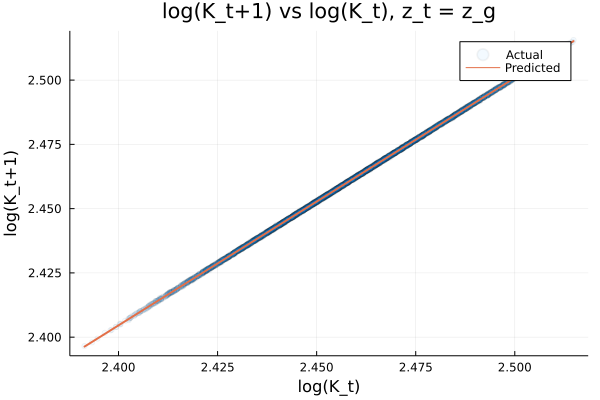
\includegraphics[scale=0.4]{gplot.png}
\end{center}
The next figure shows the observed data and regression line for $z_t = z_b$:
\begin{center}
    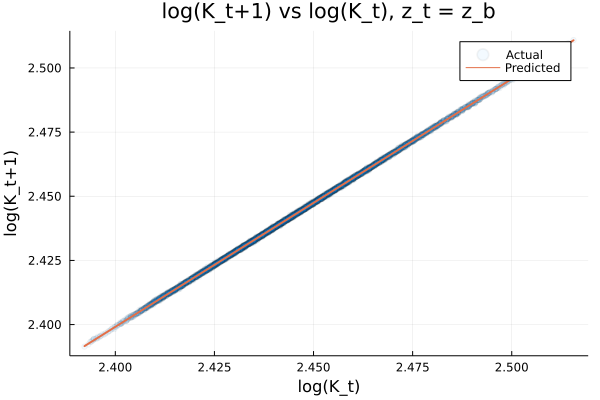
\includegraphics[scale=0.4]{bplot.png}
\end{center}
It is evident that the prediction fits quite well.

We also plot the evolution of aggregate capital from $t = 1$ to $t = 11,000$:
\begin{center}
    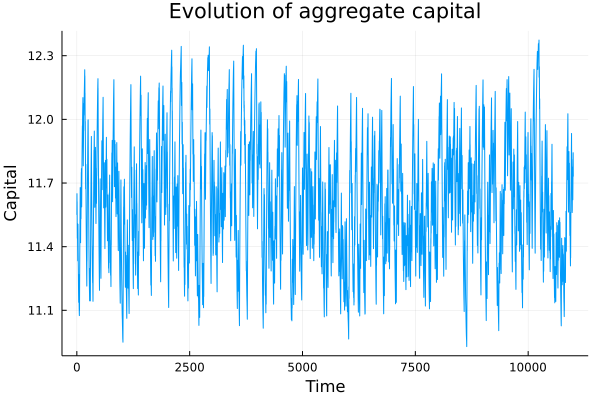
\includegraphics[scale=0.4]{akplot.png}
\end{center}
This is a very spiky boi. We can see that the aggregate capital holdings do follow an autoregressive process, as predicted.

Finally, as if we weren't having enough fun, we plotted the evolution of capital holdings for an individual agent (I chose Agent 86, for no good reason) and compared with aggregate capital:
\begin{center}
    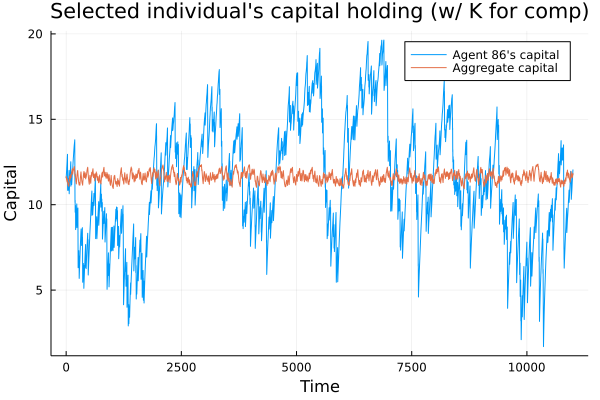
\includegraphics[scale=0.4]{indiv_plot.png}
\end{center}

\end{document}
